\section{Decision Tree}
In this section, we will discuss how the \class{DecisionTreeClassifier()} model is implemented and how the hyperparameters are chosen, as well as the results of using this model.\\

A decision tree is a supervised machine learning model that can be used for classification or regression tasks.
It works by building a tree-like structure, where at each internal node, the algorithm evaluates all the available features and selects the split that maximizes the purity of the resulting splits.
This process is repeated until a stopping condition is reached, such as a maximum depth or no further improvement in purity.
The resulting leaf nodes are also known as decision regions, and the prediction for a sample is made by traversing the tree to find the correct decision region and then predicting the most common class in that region.
Decision trees are popular because they are easy to understand and interpret due to their tree-like structure, and they can handle different types of data and decision boundaries.
However, during training, the algorithm only considers the best split for each internal node without considering the potential negative effects on future splits, which is known as a greedy approach, and can potentially lead to sub-optimal trees for some datasets.

\begin{figure}[H]
    \centering
    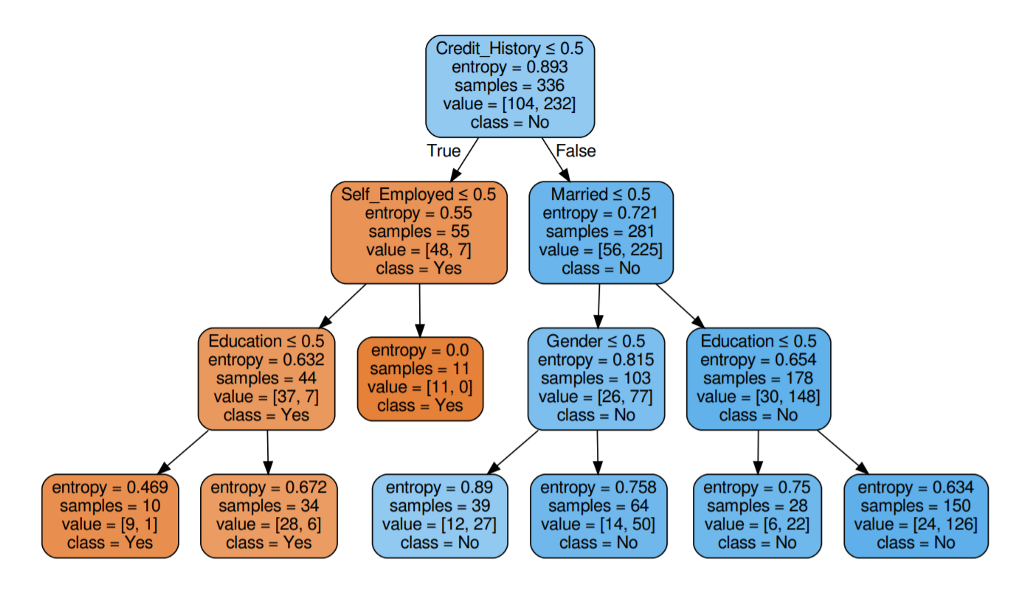
\includegraphics[scale=0.25]{figures_for_report/example_decision_tree}
    \captionsetup{justification=centering,margin=2cm}
    \caption{Simple Decision Tree}
\end{figure}


\subsection{Implementation}
As this project is focused on classification rather than regression a classification tree was implemented.
It was done in Python using two classes:\\
\begin{enumerate}
    \item \class{Node()}
    \item \class{DecisionTreeClassifier()}
    \end{enumerate}
\vspace{10pt}

\subsubsection{Node()}
The \class{Node()} class represents the internal and leaf nodes that make up the decision tree.
The \class{Node()} has the most responsibility of the two classes.
It holds the data and passes it down the tree constantly splitting itself into more nodes with the \code{_split()} method.
This is done by finding the best split with the \code{_get_best_split()} method based on either the gini or entropy impurity measure.
The term 'best split' refers to the process of selecting the feature and value that will result in the highest increase in the purity of the resulting nodes when splitting a node in the tree.
The best split of a given \code{Node()} can then be used to create two new nodes \code{self.left} and \code{self.right}.


\subsubsection{DecisionTreeClassifier()}
The \class{DecisionTreeClassifier()} is the classifier class.
which has the \code{fit()} and \code{predict()} methods and two additional  methods \code{get_depth()} and \code{get_n_leaves()}, that can be called after the model has been fitted, to get the depth and number of leaf nodes of the resulting decision tree.
The \code{fit(X, y)} method takes the following two parameters, a feature matrix \code{(X)} and class labels \code{(y)}
This data fed into the first node in the tree (the root).
The purity of the node is then found and if a split can improve the purity and all split criteria (\code{max_depth} and \code{min_samples_split}) are fulfilled the node calls \code{_split()} on itself.
This happens recursively and is how the tree-structure is created.
The \code{predict(X)} method takes an array of samples or a single sample, and predicts the corresponding label.
It works by traversing down the tree until a leaf node is reached, and then predicting the most frequent class in that node.
The constructor take the following 4 parameters.\\
\begin{itemize}
    \item \code{max_depth} - (An integer - the maximum depth to which the tree can grow)
    \item \code{min_samples_split} - (An integer - minimum number of samples in a node before for it to split)
    \item \code{criterion} - (A string - impurity measure (gini or entropy))
    \item \code{random_state} - (An integer - set the random seed for reproducible results)
    \end{itemize}
\vspace{10pt}

\subsection{Correctness}
To validate the correctness of our implementation a thorough comparison with the Scikit-learn version was done.
First a comparison of 200 Scikit-learn models and 200 of our models accuracy score was done using the \code{load_digits()} dataset from \code{Scikit-learn.datasets}, with a training and test size of $80\%$ and $20\%$ respectively.

\begin{figure}[H]
    \centering
    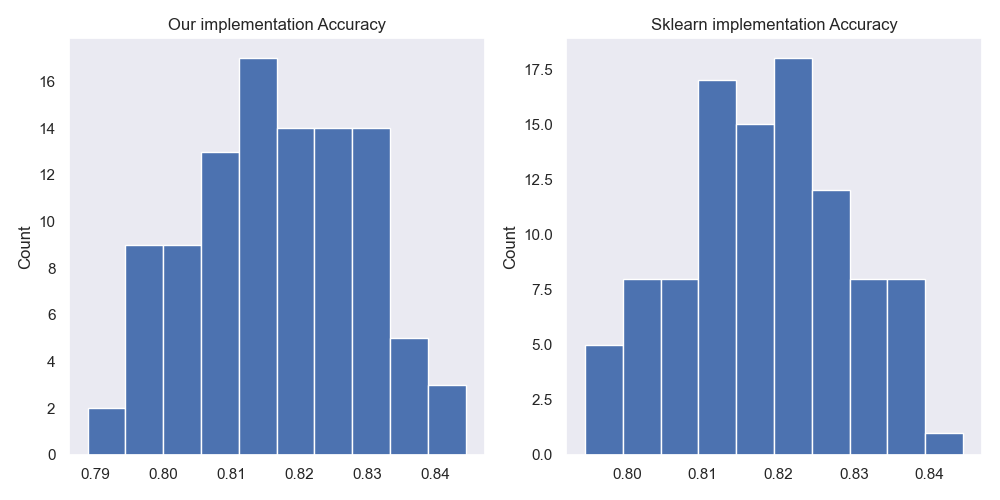
\includegraphics[scale=0.55]{figures_for_report/our_vs_sklearn_accuracy}
    \captionsetup{justification=centering,margin=2cm}
    \caption{Accuracy distribution from 200 models}
\end{figure}

Each decision tree used in Figure 5 is fitted with the default parameters of both the Scikit-learn and our model.
This means that the \code{max_depth} is not restricted and the \code{min_samples_split} is set to 2.
A decision tree has randomness involved in the training process.
This is because if two splits yield the same purity gain, one of them is chosen at random.
This means the models might perform slightly different based on a single evaluation but very similar on average as seen in Figure 5.\\

The resulting tree depths and number of leaves were also compared and showed that the decision trees in both implementations grow to the same
depth and with the same number of leaf nodes.
\\

Lastly a comparison of \textbf{some} of the actual splits (best feature and cutoff) were done to assert correctness and as a sanity check, and
the two implementations also agreed on this.\\

\subsection{Hyperparameters}
A decision tree is extremely prone to overfitting to the training data.
This is especially the case if the max depth or other early stopping to the growth is not controlled.
This can lead to a very high training accuracy but might struggle with unseen data.
Another way to solve this is using post-pruning where the tree is first grown fully, and then afterwards its size is reduced.
Post-pruning was not implemented, instead, we focused on identifying an optimal combination of \code{max_depth}, \code{min_samples_split}, and \code{criterion} (gini or entropy).
This was done using 5-fold cross-validation through the Scikit-learn class \class{GridSearchCV()}.
The following parameter grid was specified and passed to the \class{GridSearchCV()} instance.

\begin{center}
    \begin{minipage}{3in}

\begin{itemize}
    \item \code{max_depth}: [None, 5, 7, 9, 11, 12]
    \item \code{min_samples_split}: [2, 4, 8, 10]
    \item \code{criterion}: [gini, entropy] \\
\end{itemize}
            \end{minipage}
\end{center}


This led to the following combination of hyperparameters\\
\begin{tcolorbox}[colback=white,
                  arc=0pt,
                outer=0pt]
\centering \code{max_depth=9} \, \, \code{min_samples_split=4} \, \, \code{criterion=gini}\\
   \end{tcolorbox}

These values were selected due to their ability to effectively prevent overfitting, due to achieving the highest validation accuracy score.

\subsection{Results}\label{subsec:results}
\begin{table}[!ht]
\begin{subtable}[c]{0.4\textwidth}
\footnotesize
\centering
\begin{tabular}{ c | c }
 \toprule
 Evaluation Metric & Accuracy Score  \\
 \midrule
 Training Accuracy &  89.83\% \\
 Test Accuracy &79.32\% \\
 \bottomrule
\end{tabular}
\captionsetup{justification=centering,margin=1cm}
\end{subtable}
\begin{subtable}[c]{0.6\textwidth}
\footnotesize
\centering
\begin{tabular}{c | c c r}
Class & Precision & Recall & F1-Score\\
\midrule
T-shirt/Top   &    0.76  &    0.75  &    0.75 \\
Trousers   &    0.97  &    0.92  &    0.95 \\
Pullover   &    0.80  &    0.83  &    0.81\\
Dress   &    0.82  &    0.88  &    0.85\\
Shirt   &    0.61  &    0.60  &    0.60\\
\end{tabular}
\captionsetup{justification=centering,margin=1cm}
\end{subtable}
\caption{Decision Tree Performance}
\label{tab:dt_evaluation}
\end{table}\\

The results in \textbf{Table 2} are from an instance of our implementation of the \class{DecisionTreeClassifier()} with the hyperparameters specified in section \textbf{4.3}.
To reproduce these exact results it should additionally be initialized with \code{random_state=42}, to eliminate the randomness. \\

The \class{DecisionTreeClassifier()} achieved a test accuracy of $79.32\%$ and training accuracy of $89.83\%$.
Furthermore, our model emphasizes the difficulties in correctly classifying shirts, as seen by the precision, recall and f1-score.
This fits well with the feature overlap seen in \textbf{Figure 3}.
On the other hand, the model performs well at classifying the other classes especially trousers.







